\chapter{Details of the Monte Carlo Code}\label{chp:chp2}

%\begin{flushright}
%  {\em QUOTE GOES HERE }\\
%
%\ \
%
%\normalsize
%{AUTHOR}  
%\end{flushright}


\section{Monte Carlo Methods}
	 
	 \noindent{The name 'Monte Carlo' describes a class of modelling techniques that employ a stochastic approach to simulating mathematical and physical situations that are otherwise difficult or impossible to solve.  By repeatedly sampling random numbers from a probability distribution, numerical results to non-analytic problems may be obtained.  The approach was first used by researchers at Los Alamos in the late 1940s who adopted the method to model the transport of neutrons.  It is from the code name for this project, 'Monte Carlo', that the methods derive their name.  }
	 
	 As the available computing power increased over the following decades, Monte Carlo methods became more and more useful as a means of solving complex problems and are now used widely across numerous fields including mathematics, statistics, engineering, finance, the physical sciences and many others.  The nature of the approach means that they are particularly well-suited to problems with multiple degrees of freedom, and especially when any of these degrees are coupled.  By using random numbers to represent quantities that parametrise a physical problem, a model may be generated that simulates a solution to the problem using a pseudo-random number generator.   It must be the case that the quantities that characterize the problem may be represented by a continuous distribution in the range [0,1] in order that randomly generated numbers may be translated into physical properties.  
	 
	 For each randomly-generated input, the model of interest is applied and an output - a 'possible outcome' - is obtained.  By iterating this process many times with randomly-generated inputs each time, many possible outcomes are generated and a probability distribution may be built up.  The interpretation of the outputted probability distribution is dependent on the manner of utilisation of the Monte Carlo method.  For example, the iterative procedure may be used to determine best-fitting parameters of a model or may be used to find the mean-free path of a photon.  In the former case, the multi-dimensional probability distribution may be analysed to determine the most representative model or models whereas in the latter case the probability distribution is equivalent to an energy distribution.
	 
	 Clearly, Monte Carlo simulations are limited by their finite nature and will never produce a perfect solution.  However, this does not mean that Monte Carlo simulations are lacking in rigour.  It may be shown that the error in a Monte Carlo model is approximately $\sim \frac{1}{\sqrt{n}}$ for large $n$, where $n$ is the number of quanta used in the simulation.  The error may therefore be made as small as required by increasing the number of quanta used in the simulation subject to the restrictions of computing time and expense.
	 
	 In the next section, I discuss the use of Monte Carlo methods as applied to radiative transfer problems and  specifically to DAMOCLES.  I discuss the computational aspects of my work and the architecture of the code in section \ref{damocles_struct} before finally discussing the limitations of the code and its potential for future developments in section \ref{limitations}.
	 
\section{Radiative Transfer and the Monte Carlo Method}
\label{rt}

 The application of Monte Carlo codes to radiative transfer problems in astrophysics has a strong history.  Numerous codes that utilise this stochastic methodology have been written in the past few decades in order to model the transport of photon packets through various media.  The energy to be transported throughout the region of interest is discretised into packets and the path of each packet is calculated according to the properties of the environments that it passes through during its lifetime.  Collating the escaped packets at the end of the simulation produces an energy distribution. 

There exist several Monte Carlo radiative transfer codes that use this technique in order to model the transfer of line emission through a nebula to produce a synthetic spectrum. There also exist a number of codes that treat the continuous emission and absorption of energy in dusty environments in order to produce and fit a spectral energy distribution (SED).  Models of supernovae have been produced using both approaches and well-fitting spectra and SEDs have been generated but never, according to the best of my knowledge, has the mechanism been employed to produce sophisticated models of line profiles in expanding dusty regions.  In this new code, we seek to apply the technique to an expanding dusty medium in order to consider the effects on a single emitted line profile.

Previous work by Leon Lucy has considered the problem of dust-induced asymmetric line profiles in the ejecta of supernovae and he has published results derived both analytically and using simple Monte Carlo simulations.  These simulations appear to be the only published instances of a numerical approach to studying this spectral feature.  The DAMOCLES code adopts the same technique as the original modelling by Leon Lucy but allows for a considerably more complex treatment of the composition, geometry and motion of the dusty medium.

Radiative transfer methods as applied to supernovae generally treat a wide wavelength range and seek to conserve the total energy.  In the case of SED modelling, this is often achieved by dividing the total energy into packets of equal weight and energy, and iteratively determining the temperature and ionization structure.  In this work, the approach we adopt is somewhat simpler as only a very narrow wavelength range need be considered.  Rather than seeking to conserve the total energy, we assume that any packet absorbed by dust would be re-emitted outside the wavelength range of interest and thus no longer contributes to the resulting line profile.  Any absorbed packet is therefore removed from circulation.  In addition to this, the absorption and scattering of radiation by dust is independent of temperature and there is therefore no need to calculate temperatures throughout the nebula.  Similarly, in the case of radiative modelling of synthetic spectra of the ejecta of supernovae, approximations such as the Sobolev approximation are often employed to handle the blending of lines more efficiently.  This is unnecessary here as only a single line or doublet is ever treated and a comparatively narrow wavelength range considered. 

The subtleties of the problem we consider here lie in the treatment of an atmosphere expanding as fast as 10\% of the speed of light.  Lorentz transforms must be carefully applied in order that packets experience the appropriate degree of frequency shifting at emission and at each subsequent scattering event.  In this respect, the code is analogous to Monte Carlo radiative transfer models of electron scattering published by \ref{}.  Indeed, similar features are observed in the outputs of both.

Throughout this section, I will describe the principles, assumptions and techniques adopted in the production of the DAMOCLES before I move on to address the mechanics and architecture of the code itself.  DAMOCLES stands for \textbf{D}ust-\textbf{A}ffected \textbf{M}odels \textbf{O}f \textbf{C}haracteristic \textbf{L}ine \textbf{E}mission in \textbf{S}upernovae.
 

	\subsection{Energy Packets}
	
	The fundamental principle underlying the transport of radiation throughout a dusty nebula is that the radiation be discretised into packets.  Each of these packets is then propagated throughout the nebula and ultimately contributes a fraction of the final energy distribution.  At the start of the simulation, each packet is assumed to consist of $n$ photons of frequency $\nu_0$, the rest frequency of the line to be modelled.  All packets therefore begin life with initial energy

\begin{equation}
	E_0=nh\nu_0
\end{equation}
	
	
	where $h$ is Planck's constant.  As the packets move through the ejecta, they are scattered off high-velocity dust grains and after each scattering event, the frequency of the packet is altered.  In Monte Carlo simulations that model non-moving atmospheres, packets are usually taken to be of constant energy.  When the frequency of a packet is altered after an event, the energy of that packet is kept constant and the number of real photons contained within it assumed to change.  However, in the case of dust scattering, the number of real photons is conserved and thus the energy of the packet is altered.  This is most easily achieved by weighting each packet over all scattering events as 
	
\begin{equation}
	w=\prod_{scat} \frac{\nu'}{\nu}
\end{equation}

\noindent where $w$ is the weight of the packet.  The final energy of each packet is then $E =w E_0$, where $E_0$ is the initial energy of the packet.  The final dust-affected line profile is compiled by adding the total energy of all packets in a specific frequency bin in order to produce a histogram.
	
	In these models, unlike fully self-consistent SED radiative transfer models, there is no requirement that the total energy be conserved.  We drop this traditional requirement since radiation that is absorbed by dust is re-emitted outside of the wavelength range of interest and thus no longer contributes any flux to the resulting line profile.  Packets that are absorbed may be safely removed from the simulation.
	
	\subsection{Initialisation and the Grid}
	
	The supernova ejecta is approximated by a three-dimensional cartesian grid, each cell of which is assumed to have uniform density and composition.  By default, the ejecta occupies a shell between inner radius $R_{in}$ and outer radius $R_{out}$. The grid extends from $-R_{out}$ to $+R_{out}$ in each of the three axes.  Each side is split into the same number of divisions and thus each cell is a cube of volume $R_{out}^3/n_{div}^3$ where $n_{div}$ is the number of divisions along each axis and is specified by the user.  For the remainder of this thesis, a spherically symmetric situation is assumed and in all modelling and testing the grid is constructed in this manner.  However, there are no assumptions of symmetry in the code and a cartesian grid was adopted in order to allow for arbitrary geometries to be modelled in the future e.g. ellipsoidal or toroidal ejecta distributions.
	
	  Both gas and dust are by default assumed to have a power-law distribution declared as  $\rho(r) \propto r^{-\beta}$ between $R_{in}$ and $R_{out}$.  The distribution of gas determines the emissivity distribution and thus the starting positions of the packets in the simulation (see section \ref{sctn:em_prop}).  However, after the initial emission of energy packets, the gas plays no further role in the simulation as only interactions with dust grains are of interest here.  By default, the dust is coupled to the gas and thus follows the same smooth power-law distribution previously described with exponent $-\beta$.  The dust density in each cell is therefore calculated as
	
\begin{equation}
\rho (r)= \frac{M_{tot}(3-\beta)}{4\pi (R_{out}^{3-\beta}-R_{in}^{3-\beta})}
\end{equation}
	
	
\noindent where $r$ is the radial distance from the centre of the cell to the origin and $M_{tot}$ is the total desired dust mass to model.  Any cell whose centre falls outside of the bounds of the supernova ejecta has dust density set to zero.  If the dust and gas are decoupled then the user must specify distinct profiles for the gas and the dust; that is, separate power laws must be declared and independent inner and outer radii specified.  This allows for more sophisticated modelling of, for example, circumstellar shells or dense cores of dust formation surrounded by more diffuse gas.

It is known from SED modelling that clumped environments produce very different results to environments assumed to have a smooth distribution of dust and gas.  Generally, in comparison to smooth models, clumped models tend to require more dust in order to reproduce a similar level of emission or absorption.  The capacity for modelling a clumped dusty medium is therefore included in the code.  The fraction of the dust mass that is in clumps is declared ($m_{frac}$) and the total volume filling factor of the clumps ($f$) is also specified.  Dust that is not located in clumps is distributed according to a smooth radial profile.  The clumps occupy  a single grid cell and their size can therefore be varied by altering the number of divisions in the grid.  They are distributed stochastically with probability of a given cell being a clump proportional to the smooth density profile (i.e. $p(r) \propto r^{-\beta}$).  The density of all clumps is constant and is calculated as 

\begin{equation}
\rho_{clump}=\frac{M_{clumps}}{V_{clumps}}=\frac{m_{frac}M_{tot}}{\frac{4}{3} f\pi (R_{out}^{3}-R_{in}^{3} )}
\end{equation}

\noindent where $M_{tot}$ is the total dust mass, $M_{clumps}$ is the total dust mass in clumps and $V_{clumps}$ is the total volume occupied by clumps.  $m_{frac}$ and $f$ are defined as above.
	
A grid of cubic cells of varying dust and gas densities is thus produced in readiness for packets to be transported through it.  A frequency grid is also established centred on the rest-frame frequency of the line to be modelled.

	
	\subsection{Properties of the Dusty Medium}
	Dust of any composition may be used for which optical data is available.  The relative abundances of the species must be declared in an input file accompanied by a grain size distribution for each species.  Files detailing the optical data ($n$ and $k$ values) for the chosen dust species are also declared at the start of the code.  For each frequency and grain size pair, a Mie scattering routine uses this data to calculate the overall $Q_{abs}(\nu)$ and $Q_{sca}(\nu)$ by summing over the weighted grain sizes and species.  This value is then used in the calculation of the opacity of each grid cell, which determines the fate of any packets passing through it.  A Mie scattering routine is an appropriate approximation in this instance as it applies in the case of spherical scatterers where the diameter of the sphere is of the same order as the wavelength of the interacting photon.  The wavelengths of the lines of interest for this code (particularly 6563 \AA \:H$\alpha$ and 6300 \AA \:[OI])  are in the optical and near-IR  and wavelengths are therefore of the order of 0.3-1.0$\mu$m, as are dust grain radii.
%!!!! GO INTO MORE DETAIL ABOUT MIE SCATTERING AND REPHRASE THIS SECTION
	


	\subsection{Emission and Propagation}
	\label{sctn:em_prop}
	The initial radiation field is inherently tied to the distribution of gas throughout the supernova ejecta.  The relationship between the emissivity and the gas density may vary under different regimes and therefore the emissivity distribution is also specified as a power law with $i(\rho) \propto \rho^{k}$.  In general, however, this is taken to be $i(r) \propto r ^{-2\beta}$ since the majority of lines modelled are recombination lines and therefore $i(\rho) \propto \rho^2$.  The supernova ejecta is divided into shells between $R_{in}$ and $R_{out}$ and the number of packets to be emitted in each shell calculated according to the specified distributions.  For each packet a location within the appropriate shell is determined by randomly sampling from an isotropic distribution.  Three random numbers in the range [0,1) are sampled and these are translated into spherical coordinates as 

%\begin{equation}
	\begin{align}
		\phi&=2\pi\eta \\
		\theta&=\arccos(2\xi -1) \\
		r&=R_i+\zeta(R_{i+1}-R_i)
		\label{eqn:isotropic}
	\end{align}
%\end{equation}

\noindent where $\eta$, $\xi$ and $\zeta$ are random numbers, $\phi$ is the azimuthal angle, $\cos \theta$ is the radial direction cosine and $R_i$ is the inner boundary of the $i$\textsuperscript{th} shell.  At emission and at every subsequent scattering event, the packet is propelled with a new direction vector which is sample from an isotropic distribution.  I do not include forward-scattering matrices in the code since the effects of forward scattering by dust are so small as to be negligible and it is simpler and more efficient simply to assume isotropic scattering.  Having calculated an emission location, an initial propagation direction vector $(\theta,\phi)$ must be obtained.  This is calculated in exactly the same manner as described in equation \ref{eqn:isotropic} but for two newly generated random numbers.

Once a packet has been emitted into the nebula, it must be propagated through the grid until it escapes the outer bound of the ejecta $R_{out}$.  If it is not absorbed, its trajectory must be calculated and its weighting updated as it undergoes repeated scatterings.  In each cell that a packet passes through, a test is performed to determine whether the packet passes through that cell and into the next of whether it experiences an event, either scattering or absorption.  I calculate this by considering the probability that the packet travels a distance $l$ without interacting as 

\begin{equation}
p(l)=e ^{-n \sigma_{\nu} l}=e ^{-\tau_{\nu}} 
\end{equation}

\noindent where $n$ is the number density, $\sigma_{\nu}$ is the cross-section of interaction at frequency $\nu$ and 

\begin{equation}
 \tau_{\nu} = n\sigma_{\nu} l = \rho \kappa_{\nu}  l
 \end{equation}
 
 \noindent for constant $n$ and $\sigma_{\nu}$ (as in a grid cell).  The probability that a packet \textit{does} interact within a distance $l$ is therefore $1-e^{-\tau_{\nu}}$.  We may sample from the cumulative probability distribution to give: 

\begin{align}
\xi &= 1 - e^{-\tau_{\nu}}  \\
\implies  \tau_{\nu}&=-\log (1-\xi) 
\end{align}

\noindent where $\xi \in [0,1)$ is a sampled random number equivalent to the value of the optical depth for that packet in that cell.  The frequency of the photon packet and the mass density of the cell are then used to calculate the opacity of that cell and, using the fact that $n\sigma_{\nu}=\kappa_{\nu}\rho$, the distance $l$ that the packet travels before its next interaction is calculated.  If this value is greater than the distance from its position to the edge of the cell then the packet is moved along its current trajectory $(\theta,\phi)$ to the cell boundary and the process is repeated.  Alternatively, if the displacement is not sufficient for the packet to escape the cell then an event occurs.  The packet is either scattered or absorbed with probability of scattering equal to the albedo of the cell

\begin{equation}
	\omega=\frac{\sigma_{sca}}{\sigma_{sca}+\sigma_{abs}}
\end{equation}

If the packet is absorbed then it is simply removed from the simulation as discussed above.  If the packet is scattered then a new trajectory is sampled from an isotropic distribution in the comoving frame of the dust grain and the frequency of the packet recalculated using Lorentz transforms as described in the next section.  This process is repeated until the packet has either escaped the outer bound of the supernova ejecta or been absorbed.  Escaped packets are added to frequency bins weighted by $w$ in order to produce an overall emergent line profile.


	\subsection{Doppler shifting}
	
At emission and at each scattering event the frequency of the packet is recalculated according to a radial velocity field 
	
\begin{equation} 
	v(r) = v_{max}\frac{r^{\alpha}}{R_{out}^{\alpha}}
\end{equation}

\noindent where the maximum velocity, $v_{max}$, at the outer edge of the ejecta and the exponent of the velocity profile, $\alpha$, are declared in the input file.	
		
It is worth noting that if a constant mass loss rate is required, the exponent of the velocity profile and the exponent of the density profile are not independent.  A constant mass loss rate implies that $4\pi \rho vR^2  \propto k$, where $k$ is a constant, and thus for $v \propto r^\alpha$ and $\rho\propto r^{-\beta}$, we require that $\beta-\alpha=2$.  However, it is possible that the supernova event may have induced a mass-flow rate that is not constant with radius and thus both exponents may be declared independently.  It is also worth noting that for supernovae in their free expansion phase, as the majority are by the time of the onset of dust formation, the ejecta are expanding with a $v \propto r$ Hubble law expansion.
	
The outflow velocities in supernovae are extremely high of the order of 10\% of the speed of light.  Escaping radiation is therefore subject to significant, relativistic Doppler shifting. At emission and at each scattering event, the frequency of a packet must be recalculated according to the velocity of the scattering or emitting grain.  When the packet is initially emitted, it has a frequency and a trajectory in the rest frame of the emitter. Both of these must be transformed to the observer's frame in order for the packet to be propagated through the grid.  The new direction and frequency in the observer's frame may be simply found by transforming the momentum 4-vector $\boldsymbol{P}$ which is defined as

\begin{equation}
\boldsymbol{P}=
\begin{pmatrix}
	E \\
	p_x \\
	p_y \\
	p_z \\
	\end{pmatrix} =
	\begin{pmatrix}
	h \nu \\
	h \nu x \\
	h \nu y \\
	h \nu z \\
	\end{pmatrix}
\end{equation}


\noindent We may then derive $\boldsymbol{P'}$, the momentum 4-vector in the observer's frame using the relation

\begin{equation}
	\boldsymbol{P'}=\Lambda \boldsymbol{P}	
\end{equation}

\noindent where 

\begin{equation}
	{\Lambda}=
	 \begin{pmatrix} 
	 \gamma & -\gamma \beta_x & -\gamma \beta_y & -\gamma \beta_z \\
	-\gamma \beta_x & 1+(\gamma-1)\frac{\beta_x^2}{\beta^2} & 
	(\gamma-1)\frac{\beta_x \beta_y}{\beta^2} & (\gamma-1)\frac{\beta_x \beta_z}{\beta^2} \\
	-\gamma \beta_y  & (\gamma-1)\frac{\beta_y \beta_x}{\beta^2} & 1+(\gamma-1)\frac{\beta_y^2}{\beta^2} 
	& (\gamma-1)\frac{\beta_y \beta_z}{\beta^2}\\
	-\gamma \beta_z & (\gamma-1)\frac{\beta_z \beta_x}{\beta^2} & (\gamma-1)\frac{\beta_z \beta_y}{\beta^2} 
	& 1+(\gamma-1)\frac{\beta_z^2}{\beta^2} \\
	 \end{pmatrix}
	 \\
\end{equation}
\\
\\
 \noindent and $\boldsymbol{\beta}=\frac{{\bf{v}}}{c}$,   $\boldsymbol{\beta}=(\beta_x,\beta_y,\beta_z)$,   $\beta=\lvert \boldsymbol{\beta}\rvert$ and $\gamma = \frac{1}{\sqrt{1-\beta^2}}$.
 \\

In practice, the velocities considered are low enough that it is unnecessary to consider terms of order $O(\frac{v^2}{c^2})$ and thus ${\Lambda}$ may be reduced to

\begin{equation}
	{\Lambda}=
	 \begin{pmatrix} 
	 1 & - \beta_x & - \beta_y & - \beta_z \\
	- \beta_x & 1 & 0 & 0 \\
	- \beta_y  & 0 & 1 & 0\\
	- \beta_z & 0 & 0 & 1 \\
	 \end{pmatrix}
	 \\
\end{equation}

\noindent The new direction of travel and frequency in the observer's frame are therefore given by  
\begin{equation}
\nu'=\nu(1-x\beta_x-y\beta_y-z\beta_z) \\
\end{equation}
\begin{equation*}
\begin{split}
x'=\frac{\nu}{\nu'}(x-\beta_x) \\
y'=\frac{\nu}{\nu'}(x-\beta_y) \\
z'=\frac{\nu}{\nu'}(x-\beta_z) \\
\end{split}
\end{equation*}

For each scattering event, the packet must be transformed both into and out of the comoving frame. The reverse transform is applied by using the inverse Lorentz matrix $\Lambda^{-1}$ which is obtained by reversing the sign of $\bf{v}$.  Positive $\bf{v}$ is defined for frames moving away from each other and thus $\bf{v}$ is defined to be negative in the direction of the observer.
	

	\subsection{Electron Scattering}
	As will be discussed in detail in chapter three, the effects of scattering on the shapes of line profiles can potentially be quite pronounced and it is therefore important to consider the potential effects of electron scattering as well as those of dust scattering.  A simple treatment of electron scattering calculates electron densities using an estimated average temperature of either 5000K, 10,000K or 20,000K.  An observed luminosity of $H_{\alpha}$ is then used to calculate the optical depth to electrons.  Electron scattering is treated in an identical manner to dust scattering with the overall optical depth $\tau = \tau_{dust}+\tau_{e}$ in each cell.  If, for a given packet, an event ocurrs, it is first calculated whether this is a dust event or an electron scattering event by considering the ratio of the optical depths of each species to the total optical depth.  If the packet is scattered by an electron then this process is identical to dust, but the velocity of the scatterer now has a thermal component that must be considered.  
	
	%ES CALCN HERE.

In the majority of cases it seems that the electron densities are not high enough to discernibly effect the overall shape of the profile.  However, there may be a few rare cases (the concept is discussed for SN 2010jl \citep{Fransson2013}) where the electron densities are high enough to become significant in the observed profiles.  Whilst the inclusion of electron scattering in the code is an approximation, it gives a good suggestion of the potential effects of electron scattering.	
	
	\subsection{Doublets}

One of the lines in supernovae emission spectra that is frequently seen to be blue shifted is the forbidden [OI]$\lambda$6300,6363\AA\ doublet (e.g. SN1987A \citep{LucyEtAl89} figure \ref{fig:Lucy89_87A}).  DAMOCLES therefore has the capacity to treat doublets as well as single lines.  When a doublet is specified, both the initial wavelengths and the initial intensity ratio must be declared.  The code will create a wider frequency array than for a single line in order to accommodate both lines.  It will then model each line independently, adding the final fluxes of the lines to produce the desired doublet at the end of the modelling. 

\subsection{Comparing the Model with Observations}
	
\section{The Structure of Damocles}
\label{damocles_struct}
	
	\begin{centering}
	\begin{figure}
	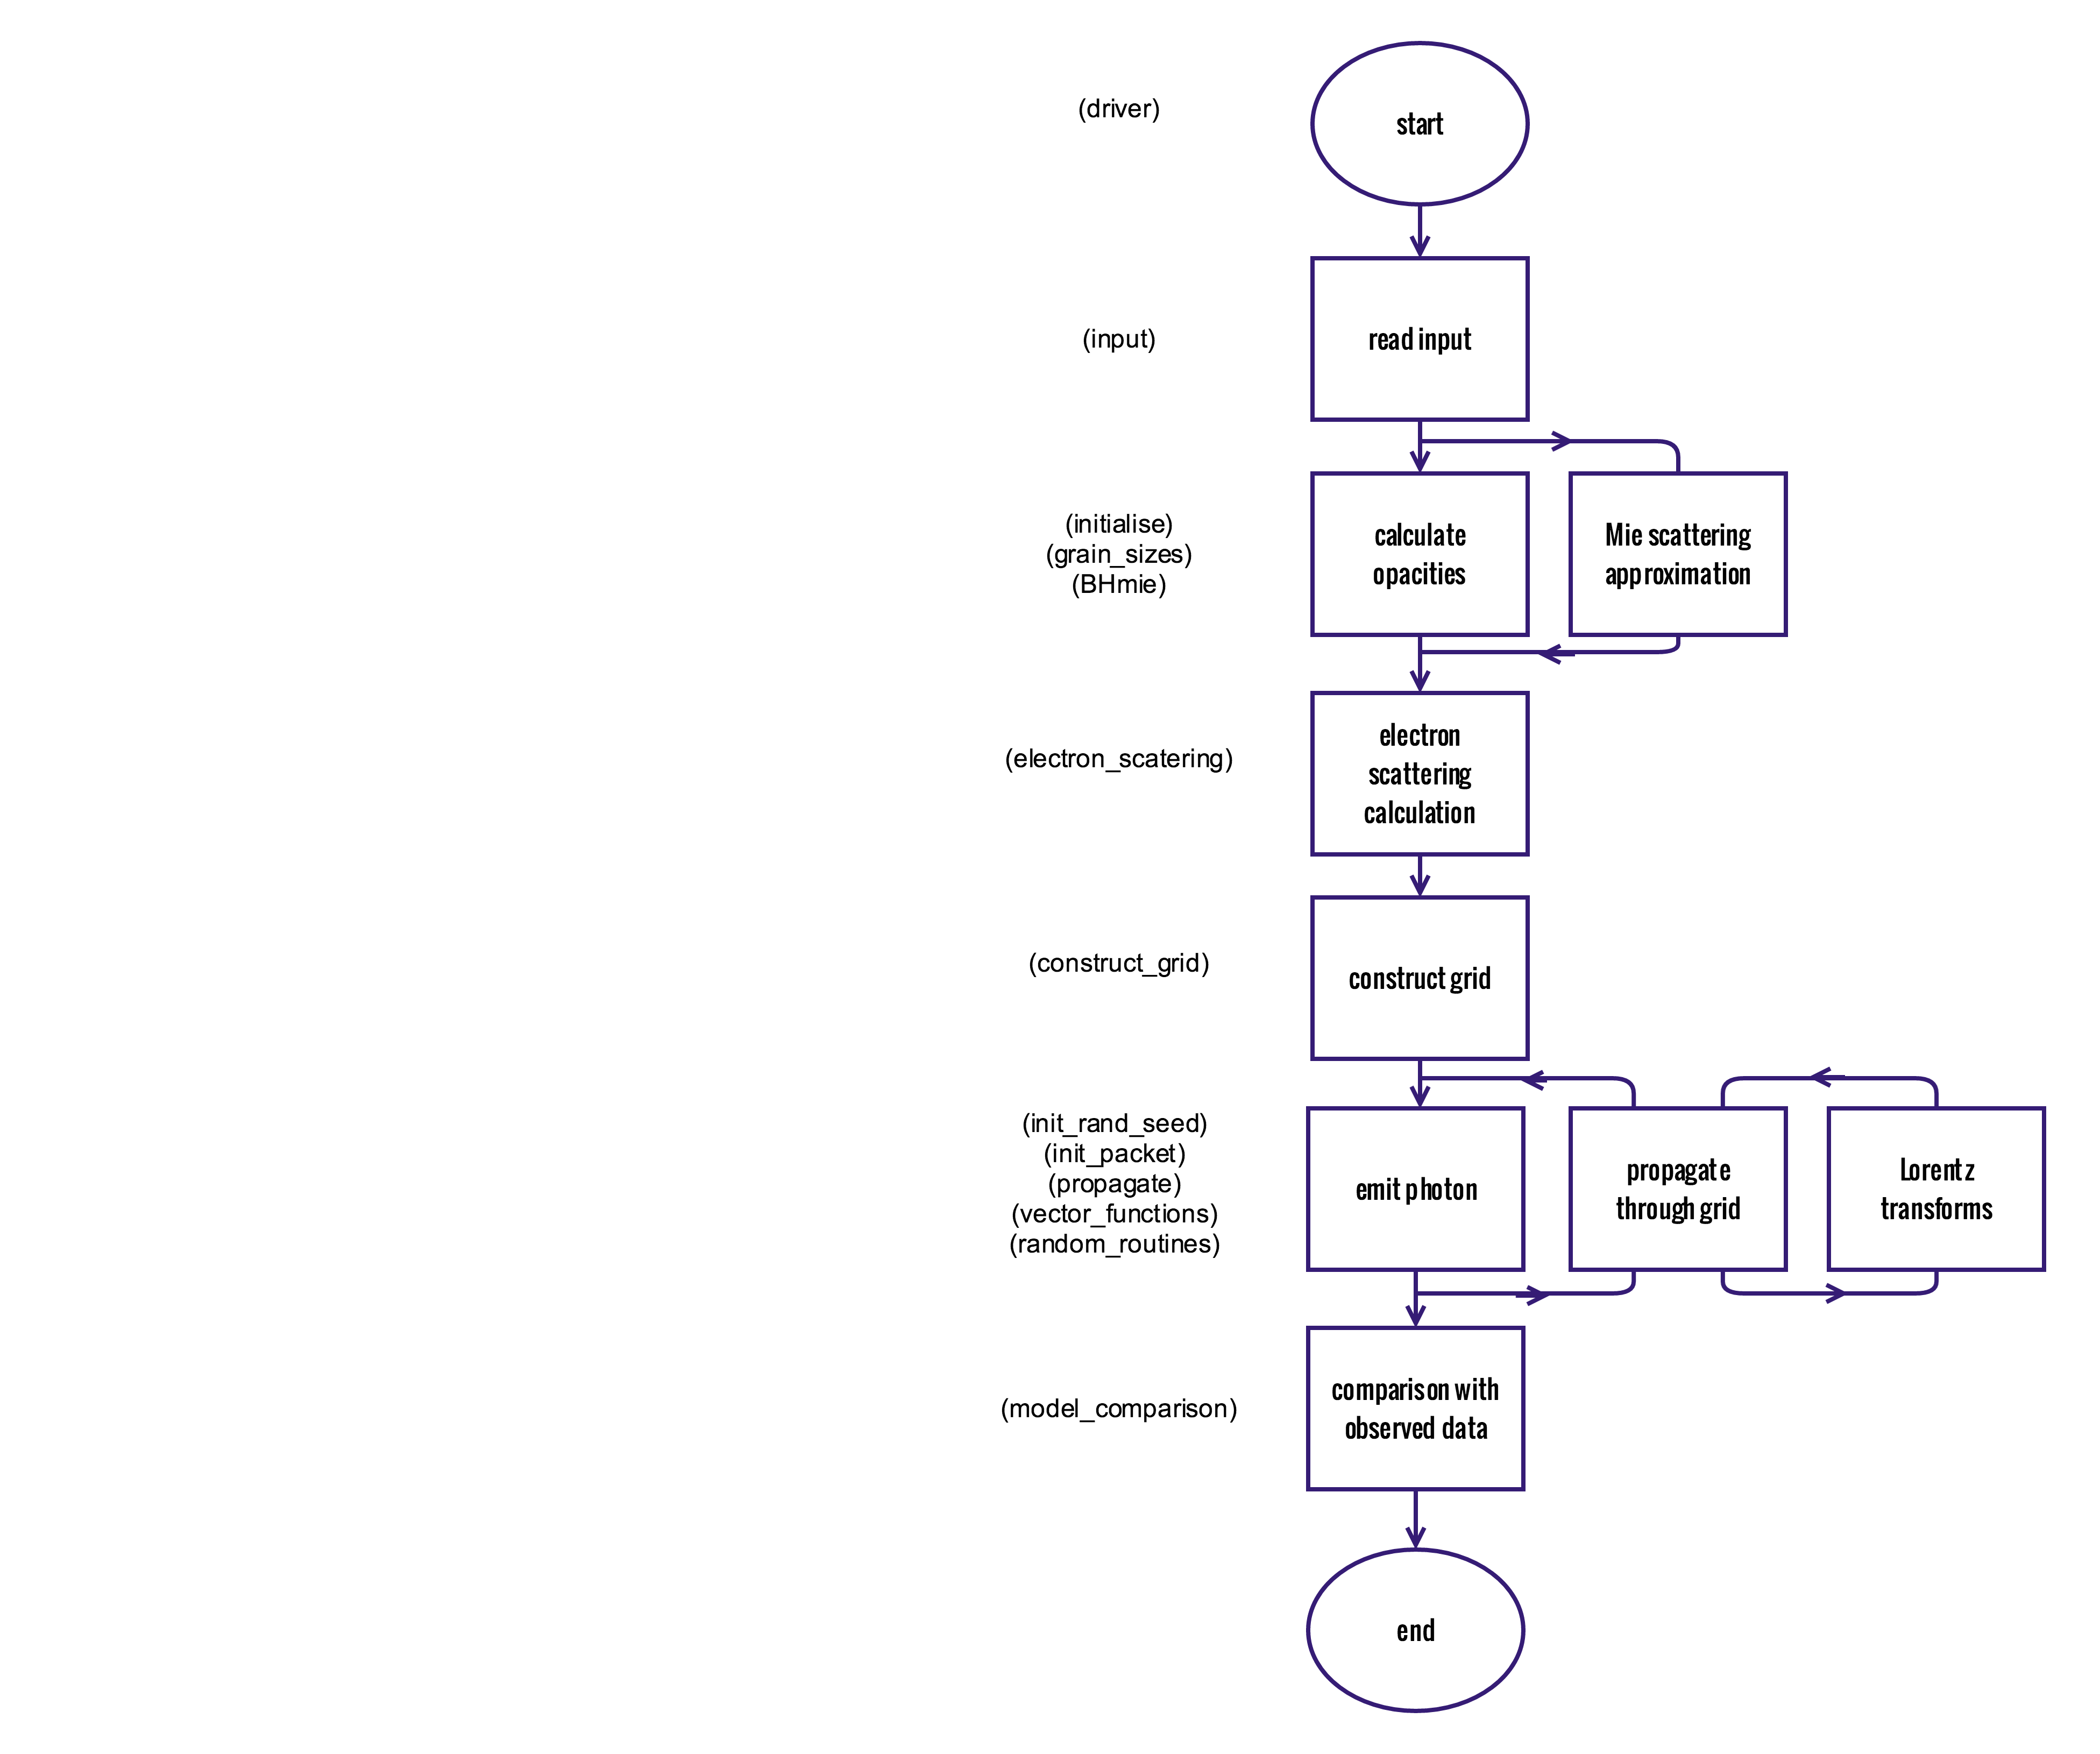
\includegraphics[scale=0.8, trim=160mm 5mm 8mm 5mm]{chapters/chapter2/code_flow.png}
	\caption{A flowchart representing the sequence of processes that take place in the Damocles code.  The modules involved at each stage are given in parentheses.}
	\label{fig:flowchart}
	\end{figure}
	\end{centering}	
	
	
	%TALK ABOUT WHY YOU USED FORTRAN 90
	\subsection{Computational Architecture and Processes}



	
	Damocles was written using a modular structure.  The "parent" driver has numerous "children" in the form of subroutines and modules which are each responsible for a separate task or tasks.  This architecture has a number of advantages.  Firstly, it serves to clarify both the functionality and legibility of the code allowing for easier debugging and maintenance.  It also allows for the implementation of features such as recursive subroutines which are ideally suited to a Monte Carlo methodology.  Finally, it allows for the code to be developed further in the future simply by including additional modules and subroutines.  A brief description of every module and subroutine in the code is presented in the following subsections.  The descriptions are ordered according to the first time they or their contents are called by the driver (see figure \ref{fig:flowchart_mods} for a flowchart of the modular hierarchy).
	

		\subsubsection{The driver}
		The \textit{driver} module is at the centre of Damocles.  It is from here that all subroutines are called.  The calls to construct the grid and calculate dust opacities, to emit and propagate packets and to compare the results with observational data are all made from here.  The parallelisation process is also controlled from here (see section \ref{scn:open_mp} for more details on the parallel function of Damocles).  Having called the initialisation routines, the driver is reponsible for dividing the ejecta into shells and calculating how many packets are emitted within each shell.  Each shell is looped over and each packet is looped over within each shell. Emission and propagation routines are called inside this loop.  At the end of each packet's lifetime, either once it has been absorbed or has escaped, the driver adds the weighted packet's energy to the appropriate frequency bin and stores this information before looping back to emit and propagate the next packet.  It is here that a line of sight is applied if so desired.  This is achieved by collecting only packets that have escaped within a cone of angle $\pi/6$.  Once all packets have been processed, the driver writes the relevant information to the output file and calls the model comparison module.  
	
		The driver is also the section of code responsible for processing doublets.  The code treats doublets by processing two batches of packets with differing initial frequency through the same grid.  Before they are collected in frequency bins, the flux ratio that is specified by the user is applied to one batch of the packets.  All packets are then collected as per a single line. 
		
		Various statistics are also processed and output here including the fraction of packets that are absorbed and the estimated undepleted luminosity of the observed line. 
		
			\begin{centering}
	\begin{figure}
	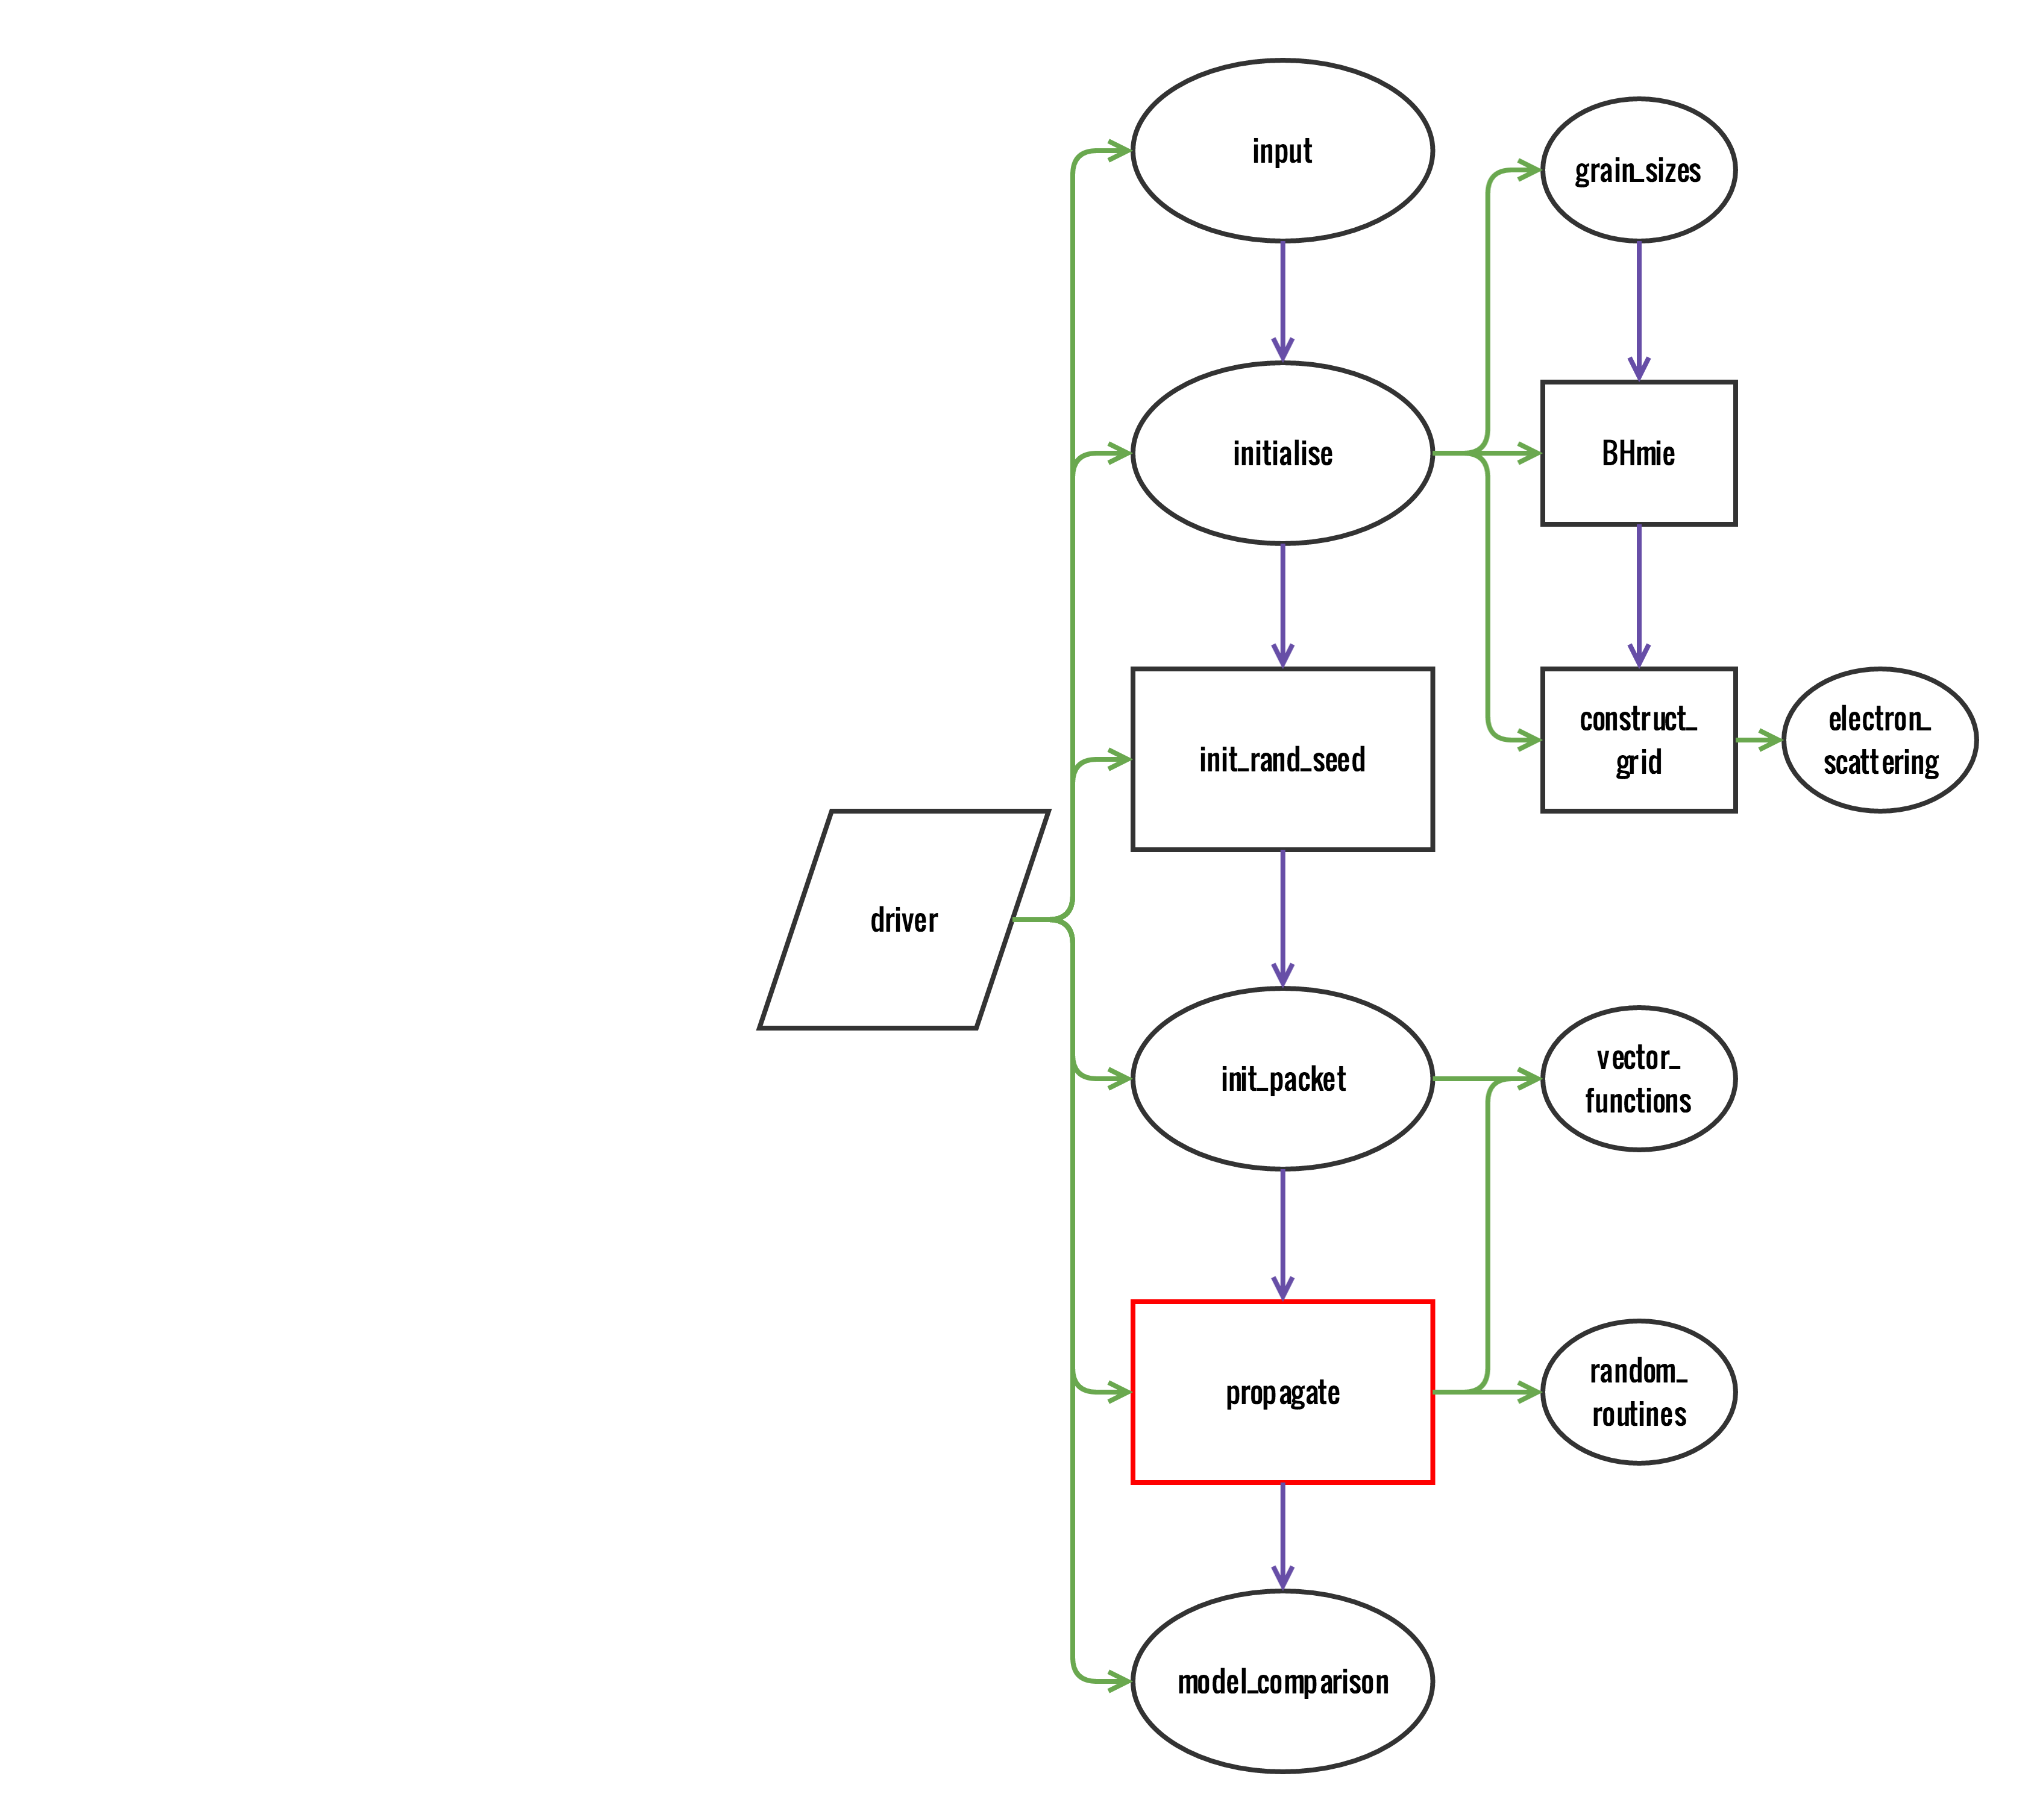
\includegraphics[scale=0.8, trim=110mm 0mm 0mm 5mm]{chapters/chapter2/code_modules_flowchart.png}
	\caption{A flowchart representing the hierarchy of modules and subroutines in the Damocles code.  Ellipses represent modules and rectangles represent subroutines (the red rectangle is a recursive subroutine).  Green arrows indicate the dependence on module or subroutine on previous modules or subroutines.  Purple arrows indicate the flow of the code.}
	\label{fig:flowchart_mods}
	\end{figure}
	\end{centering}
		
		\subsubsection{The input module}
		The \textit{input} module is where the primary input file is read into the code and all global variables are declared and assigned.  A number of logicals are assigned based on values declared in the input file and some simple calculations are performed that determine the inner and outer radii based on the maximum velocity specified and the epoch of consideration.  A number of physical constants that are used throughout the code are also declared here as 'parameters', meaning that their value cannot be changed at any point in the simulation.
		
		\subsubsection{The initialisation module}
		The \textit{initialise} module acts as a driver to run all of the subroutines associated with initialising the program.  A number of dynamically allocatable arrays are declared allowing for a grid of densities to be calculated, a frequency grid to be stored and optical properties to be read in.  Arrays to store the emergent spectrum are also declared.  The calculation of dust opacities, which calls the \textit{grain\_sizes} subroutine and the \textit{BHmie} subroutine, is performed here.  For each species, the wavelength-dependent optical properties, $n$ and $k$, are read in and the Mie approximation applied to every pair of frequencies and grain sizes.  The resulting extinction and scattering efficiencies are summed over all grain sizes for each wavelength, weighted appropriately, to calculate overall wavelength-dependent extinction and scattering opacities.  These data are stored in an array that is accessed as a packet is processed through the grid.   
		
		The command to construct the grid is called before some basic statistics about the grid are calculated.  The average optical depth from $R_{in}$ to $R_{out}$ in both the V band and the rest-frame wavelength of the line being modelled are calculated and sent to stdout.  The average number density of grains in each cells is also computed and output.  Finally, the frequency array that will divide the packets into bins is constructed.
		
		This module is also where the \textit{gridcell} derived type is declared.  A \textit{gridcell} type was specified as it allowed for easy and clear access to any of a grid cell's properties as a packet is passing through it.  The type consists of a number of arrays of real, integer and logical variables.  The properties recorded for each cell include the physical bounds of the cell in each axis, the mass and number dust densities,  the electron density, an identifying number  and a logical clumped property. 
		
		\subsubsection{The grain size module}
		The \textit{grain\_sizes} module reads in the file that specifies the list of species to be used.  This file is a list of species detailing for each one the name of the file containing the optical data for the species, the relative abundance of that species, the maximum and minimum grain sizes and the exponent of the power law of the grain size distribution.  It also declares a grain size resolution.  These properties are all read in by the \textit{grain\_sizes} module and a relative weight calculated for each grain size for each species.
		The \textit{species} is declared in this module.  As for the \textit{gridcell} type, using a derived type allowed for the easy storing and accessing of a large number of properties of each species.  Many multi-dimensional arrays and scalars were stored for the \textit{species} type that included properties relating to the grain size distribution, the density of a dust grain, the extinction and scatting opacities and the relative abundance of the species amongst others.  After processing of the optical data for a given species, all calculated quantites were stored in arrays as a component of the \textit{species} type. 
		
		\subsubsection{The Mie approximation subroutine}
		The \textit{BHmie} subroutine is a standard routine that  was obtained from an online library of routines.  It is a modified version of the Bohren and Huffman (1983) %FIX REFERENCE HERE 
		Mie scattering routine.  It applies a complex algorithm to approximate the extinction and scattering efficiencies of a single size grain at a specified wavelength given its complex refractive index $n+ik$.
		
		\subsubsection{The grid construction subroutine}
		The \textit{construct\_grid} subroutine is called from within the initialisation module.  The purpose of this subroutine is to populate the grid, which is an array of derived type \textit{gridcell} and size $n_{cells}$ where $n_{cells}$ is the number of cells in the grid.   The bounds of the grid are initialised and the radii of all cells from the centre of the grid tot he centre of the cell calculated.  The density of each cell is then calculated according to the smooth distribution and scaled so that the total dust mass is equal to that specified in the input file.  If clumps are used then the total number of clumps is calculated and these are distributed throughout the grid stochastically according to the smooth density profile stipulated.
		This subroutine also calls the electron scattering subroutine contained within the \textit{electron\_scattering} module so that the electron density of a cell may be stored at the same point as the dust density.
		
		\subsubsection{The electron scattering module}
		The \textit{electron\_scattering} subroutine  %WHAT DOES IT CALCULATE????
		
		\subsubsection{The random seed subroutine}
		The \textit{init\_rand\_seed} is a short subroutine that calculates a seed for the standard Fortran pseudo-random number generator (\textit{random\_number}).  It uses the system clock to generate the random seed and thus varies with every implementation of the code.  A seed is a number that is used as a 'starting point' for a pseudo-random number generator.  Varying the random seed ensures that a different set of random numbers is generated every time the code is run, which can be useful to ensure that any peculiar or interesting features of the code are definitely a product of the physical processes and not as a result of random fluctuations in the simulation.  The more packets are used however, the more the Monte Carlo noise in the emergent line profile is reduced and the contribution from any anomalous packets should be insignificant.
		
		\subsubsection{The packet initialisation module}
		The \textit{init\_packet} module is responsible for the creation and emission of packets at the start of the simulation.  It is called from the driver for each packet.  By generating an array of five random numbers, the position and emission direction vectors in the rest frame of the emitter are calculated according to the formulae described in equation \ref{eqn:isotropic}.  The scalar velocity of the emitter is calculated based on its radial position and this converted into a velocity vector by normalising the position vector and multiplying by the scalar velocity.  The velocity vector is passed to the Lorentz transforms subroutine contained the \textit{vector\_functions}  module.  The frequency of the packet is also passed to this subroutine.  After the emission direction vector and frequency of the packet have been updated, the grid cell in which the packet starts its path is identified and the code passes back to the driver to propagate the packet through the nebula.
		
		\subsubsection{The vector functions module}
		A number of vector functions are contained within the \textit{vector\_functions} module and are accessed throughout the simulation.  These include normalisation functions, conversions from spherical coordinates to cartesian and both forward and inverse Lorentz transforms.  It is the latter of these that is most important for the physics of the code.  The Lorentz functions are called for each packet at emission from the \textit{driver} and at every subsequent scattering event from within the \textit{propagate} routine.  As well as performing the necessary frequency shift based on the velocity of the scatterer or emitter, they also transform into and out of the rest frame of the particle thus ensuring that the packet is propagated through the nebula with a direction in the rest frame of the observer but that its new direction is sampled from an isotropic distribution in the rest frame of the influencing dust grain.  
		
		The $\beta$ and $\gamma$ values are calculated based on the input velocity vector.  The momentum 4-vector is then multiplied by the Lorentz matrix using the Fortran function \textit{matmul} to produce a  a new frequency and a new direction vector in the appropriate frame of reference.  If a scattering event has occurred then the weight of the packet is also updated here.  The new direction vector, frequency and weight are then passed back to the propagate routine and the process repeated.   At each scattering event the inverse Lorentz matrix must first be applied to move from the observer's rest frame to the particle's.  A new direction vector must then be sampled from an isotropic distribution before applying the forward Lorentz transform to move back from the rest frame of the dust grain to the observer's frame.  The next step in the packet's trajectory may then be calculated in the \textit{propagate} subroutine.
		
		\subsubsection{The propagate subroutine}
		The \textit{propagate} subroutine is at the heart of the Monte Carlo simulation.  It is here that the trajectories and experiences of all packets in the simulation are determined.  The \textit{propagate} is a subprogram called a \textit{recursive subroutine}.  This allows the subroutine to call itself, at which point it will loop back to the start of the subroutine.  It will continue this process until a condition is reached that instructs it to return to the driver.  In this case a number of conditions will arrest the circulation of the packet. If the packet has escaped the outer radius of the ejecta or has been absorbed then the routine will pass this information along with the frequency and weight of the packet back to the driver.  The routine would also stop recurring if a packet has undergone a maximum number of scattering events.  At this point it is deemed that the weight of the packet is so small as to be negligible and it is classified as 'inactive'.  This prevents the code from lagging by becoming stuck on a particular packet that has become trapped in a region of high density and albedo. 
		
		\begin{centering}
            	\begin{figure}
            	\fbox{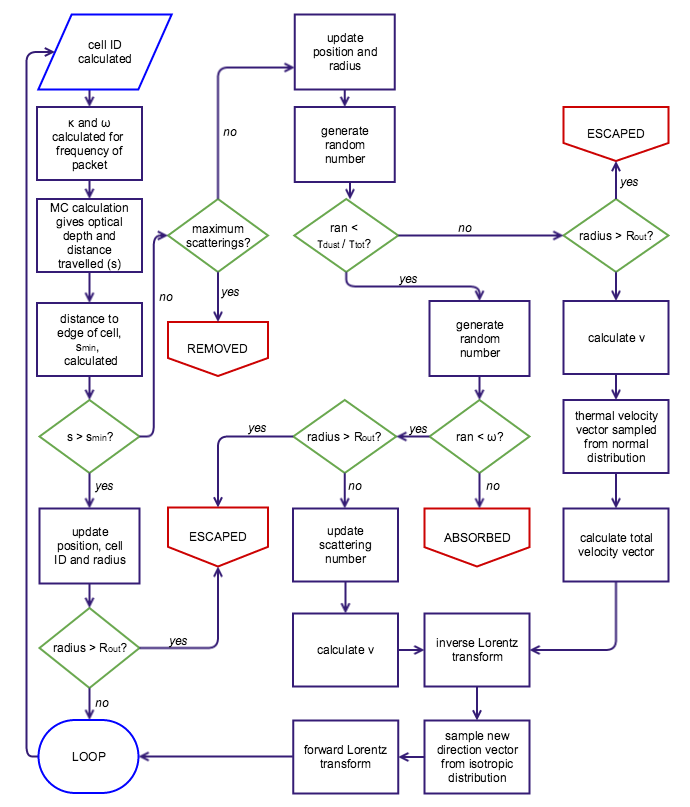
\includegraphics[scale=0.7, trim=8mm 0mm 8mm 5mm]{chapters/chapter2/propagate_module.png}}
            	\caption{A flowchart representing the }
            	\label{fig:flowchart_propagate}
            	\end{figure}
            	\end{centering}
		
		There are a number of processes that take place in this module in order to propagate a packet through the nebula accurately.  A full pictorial representation of the procedures that are implemented in this module may be found in the flowchart in figure \ref{fig:flowchart_propagate}. For each packet in each cell, the optical depth in that cell is calculated based on the opacity and density at the frequency of the packet.  These are obtained by interpolating between discrete opacities at points in the frequency array.  This is the point at which the Monte Carlo technique is applied in order to determine the distance travelled by the packet.  This displacement is then compared to the distance to the edges of the cell in order to ascertain whether or not the packet escapes the cell.  If it does then the process is repeated until either an event occurs or the packet escapes the nebula.  If an event occurs, a series of random numbers are sampled in order to determine whether or not the packet suffers electron scattering, dust scattering or absorption.  If the packet is absorbed then it is removed from the simulation.  If it is scattered then the velocity vector is calculated.  In the case of electron scattering this involves considering the thermal velocity component as well as the bulk velocity at that radius.  The Lorentz transforms are applied updating the frequency of the packet and a new direction of propagation sampled, and the routine is recalled to start afresh. 
	

		
		\subsubsection{The random routine module}
		\textit{random\_routine}
		
		\subsubsection{The model comparison module}
		\textit{model\_comparison}
	
	\subsection{OpenMP Parallelisation}	
	\label{scn:open_mp}
	
	\subsection{Input}
	
	
	\begin{table}[htdp]
\caption{The input variables read in from the input file and example values}
\begin{center}
\begin{tabular}{l r c|c l r}
\hline
Input Variable & Example Value &&& Input Variable & Example Value\\
\hline
lambda1\_0 & 636.3 &&& MD\_tot & 1.0e-4\\
L\_tot & 0.003 &&& l & 1.0\\
L\_Halpha & 0.005 &&& q & 1.3\\
doublet & 1 &&& b & 2.0\\
lambda2\_0 & 630.0 &&& gas\_shell & 1\\
L\_ratio & 3.1&&& v\_max\_gas & 8000\\
ES & 1 &&& Rrat\_gas & 0.05\\
ES\_temp & 10000 &&& l\_gas & 1.0\\
ls & 0 &&& q\_gas & 1.5\\
VelShift & 1 &&& b\_gas & 2.0\\
mf & 0.5 &&& ncells & 50\\
ff & 0.1 &&& n\_packets & 1e8\\
dayno & 680 &&& n\_bins & 1000\\
v\_max & 5000 &&& n\_shells & 100\\
Rrat & 0.2 &&& dustfile & 'species\_file.in'\\
\hline
\end{tabular}
\end{center}
\label{default}
\end{table}%
	
	\subsection{Output}
\section{Post-Processing and Visualisation}
\section{Limitations and Further Developments}
\label{limitations}

\clearpage
		


THE REST FOLLOW HERE. 


